\documentclass[a4paper]{article}
\usepackage[utf8]{inputenc}
\usepackage[slovene]{babel}
\usepackage{graphicx}
\usepackage{hyperref}
\usepackage[nottoc]{tocbibind}
\usepackage{caption}
\usepackage{subcaption}
\usepackage{amsmath}
\usepackage{ dsfont }
\usepackage{siunitx}
\usepackage{multimedia}
\usepackage{float}
\usepackage[table,xcdraw]{xcolor}
\setlength\parindent{0pt}

\newcommand{\ddd}{\mathrm{d}}
\newcommand\myworries[1]{\textcolor{red}{#1}}
\newcommand{\Dd}[3][{}]{\frac{\ddd^{#1} #2}{\ddd #3^{#1}}}

\begin{document}
\begin{titlepage}
    \begin{center}
        
\includegraphics[]{logo.png}
        \vspace*{3cm}
        
        \Huge
        \textbf{Naključna števila in integracije z metodo Monte Carlo}
        
        \vspace{0.5cm}
        \large
        7. naloga pri Modelski Analizi 1

        \vspace{4.5cm}
        
        \textbf{Avtor:} Marko Urbanč (28232019)\ \\
        \textbf{Predavatelj:} prof. dr. Simon Širca\ \\
        \textbf{Asistent:} doc. dr. Miha Mihovilovič\ \\
        
        \vspace{1.8cm}
        
        \large
        23.11.2023
    \end{center}
\end{titlepage}
\tableofcontents
\newpage
\section{Uvod}
Danes bojo pomembna naključna števila, saj bomo z metodo Monte Carlo računali integrale. 
Dobro je, da se zavedamo dejstva, da naključna števila, ki nam jih da recimo \texttt{np.random}
niso dejansko naključna, ampak so generirana po nekem algoritmu, ki je determinističen. Težko (beri: nemogoče) je
računalniku dati natančna navodila o tem kako naj nekaj nenatančno oz. poljubno naredi. Zato se poslužujemo
nekaterih algoritmov, ki nam pomagajo pri generiranju naključnih števil. V tem primeru bomo uporabili
\texttt{numpy.random.uniform}, ki nam vrne naključno število iz enakomerne porazdelitve na intervalu $[0,1)$.
To my surprise je, da \texttt{numpy} uporablja Mersenne Twister algoritem. In hindsight bi lahko vzel tudi kakšen 
preprostejši algoritem, ki bi bil hitrejši, čeprav \texttt{numpy} uporablja nekaj trikov, da je hitrejši. \\


Pri Monte Carlo integraciji naključno izbiramo točke v prostoru, kjer imamo neko omejeno območje, ki ga integriramo.
Recimo, da je to območje $[a,b] \times [c,d]$, kjer smo od tega še nekaj odrezali, da dobimo trikotnik v profilu. V takem primeru 
bi izbirali naključne točke $(x,y)$, kjer je $x \in [a,b]$ in $y \in [c,d]$ in vsakič, ko izberemo točko, preverimo, če je
znotraj območja, ki ga integriramo (v temu preprostemu primeru, ko nekaj odrežemo, preverimo ali je točka znotraj trikotne prizme).
Če je točka znotraj, potem inkrimentiramo števec, ki nam pove koliko točk je znotraj. Na koncu integriramo tako, da delimo število
točk znotraj z številom vseh točk in to pomnožimo z volumnom območja, ki ga integriramo. Tako smo dobili volumen, v našem primeru,
trikotne prizme. Če imamo neko funkcijo $f(x,y)$, ki jo integriramo, potem to funkcijo pomnožimo v vsaki točki znotraj območja, ko 
jo izberemo. To si bomo pogledali na treh primerih. 

\section{Naloga}
Danes sem zgrešil rok za oddajo in namesto, da bi imel edini prosti večer, pišem report. Posledično sem nekoliko bolj redkobeseden,
kot bi bil sicer, zato kar pojdimo na naloge.

\subsection{Zvezdasti lik}
Najprej si poglejmo zvezdasti lik, ki ga omejuje ploskev:
\begin{equation}
    \sqrt{\vert x \vert} + \sqrt{\vert y \vert} + \sqrt{\vert z \vert} = 1
\end{equation}
Naloga želi, da izračunamo maso in vztrajnostni moment tega lika v dveh primerih. Prvi primer je, ko je gostota konstantna 
in v drugem primeru, ko je gostota odvisna od razdalje od izhodišča z neko potenco $r^p$.

\subsection{Rojevanje žarkov gamma}
V drugi nalogi si zamislimo, da se v središču krogle rojevajo žarki gamma. Naloga želi, da izračunamo verjetnost za pobeg žarka
iz krogle in pogledamo, kako se ta verjetnost spreminja z povprečno prosto potjo žarkov in radijem krogle.

\subsection{Nevtronski reflektor}
V zadnji nalogi si poglejmo nevtronski reflektor, ki je pravzaprav plošča z neko debelino. Na reflektor pošiljamo tok nevtronov, ki
se v njej siplejo in absorbirajo. Naloga želi, da izračunamo verjetnost, da se nevtron, ki ga pošljemo v reflektor, pride skozi 
reflektor. Povprečna prosta pot je enaka polovici debeline reflektorja. Dodatno lahko potem stvari še malo bolj zakompliciramo in
dodamo še možnost gibanja v prečnih smereh.

\section{Opis reševanja}
Ker imam rad HPC, sem za namen naloge napisal integrator, ki je sposoben delati na več jeder. To sem naredil tako, da sem
si napisal razred \texttt{NumberNecromancer}, ki sprejme funkcijo, ki jo integriramo skupaj z območjem, ki ga integriramo in 
število točk, ki jih generiramo. Nato razred razdeli točke na več delov, ki jih lahko integriramo na različnih procesorjih. 
Točke se generirajo na vsakem procesorskem jedru ločeno, tako da je manj pošiljanja podatkov med procesorji in je manj verjetno, da 
bi zašli v težave s ponavljanjem naključnih števil. Ime inspired od tega, da rabim Necromancy, da sem še pokonci. \\

Torej s tako napisanim integratorjem je reševanje vsake naloge prevedeno na to, da pravilno napišemo funkcijo, ki jo integrator
sprejme. Jaz sem to imenoval \textit{condition function}, ker je to funkcija, ki preverja, če je točka znotraj območja, ki ga
integriramo in če je, potem nekaj z njo naredi. Integrator sem preveril prvo na primeru kroga v kvadratu, kjer sem z integracijo
izračunal $\pi$. To sem naredil tako, da sem integriral funkcijo $f(x,y) = 1$ in primerjal razmerje točk znotraj kroga in vseh
točk z razmerjem ploščin kroga in kvadrata. 

\begin{equation}
    \frac{4 N_{\mathrm{in}}}{N_{\mathrm{tot}}} \to \pi \>.
\end{equation}

Skoraj vsa integracija je potekala na mojem Ghetto clustru, kjer je bilo tokrat na voljo 152 jeder. To je bilo fino, ker 
sem lahko jemal večja števila točk in ker je lahko cluster dobil queue dela in je delal, ko sem jaz spal, čeprav as you might know,
sem spal predolgo in posledično sem zgrešil rok za oddajo. Duša je želela, telo je reklo ne. \\

\subsection{Zvezdasti lik}
Za maso zvezdastega lika sem pravzaprav integriral funkcijo $f(x,y,z) = 1$ in jo pomnožil z gostoto, ki je bila postavljena na
$1$, saj je tako ali tako konstantna. Za vztrajnostni moment pa sem integriral funkcijo $f(x,y,z) = x^2 + y^2 + z^2$. No pravzaprav
sem malce slabo prebral navodila in sem računal vrtilno količino, ampak ker je bila kotna hitrost enaka $1$, je to isto kot
vztrajnostni moment. \\

V drugem primeru, ko je gostota odvisna od razdalje od izhodišča, sem funkcijo $f(x,y,z)$ pomnožil z funkcijo 
$g(x,y,z) = (x^2 + y^2 + z^2)^p$, ki predstavlja radialni profil gostote.

\subsection{Rojevanje žarkov gamma}
Ker \texttt{NumberNecromancer} žreba točke uniformno na dani domeni (kar se sicer v splošnem lahko override-a, ampak je tako 
preprostejše) sem računal naključen radij in naključen kot takole:

\begin{gather}
    r = \xi^{1/3}\>, \\
    \theta = \arccos(2 \xi - 1)\>,
\end{gather}

kjer je $\xi$ naključno število iz enakomerne porazdelitve na intervalu $[0,1)$. Tako sem dobil naključno točko na projekciji 
krogle na ravnino $xy$. V tem primeru so bile vse točke by definition znotraj krogle. Treba je bilo še izžrebati povprečno prosto
pot takole:

\begin{equation}
    \lambda = -\frac{1}{\mu} \ln(\xi)\>,
\end{equation}

Če je bila ta daljša od razdalje $d$, potem je žarek pobegnil, sicer pa je bil absorbiran. $d$ sem izračunal kot slednje:

\begin{equation}
    d = -r \cos\theta + \sqrt{1 - ({r}/{R})^2(1-\cos^2\theta)}\>,
\end{equation}

kjer je $R$ radij krogle, ki je tako ali tako bil postavljen na $1$. \\

\subsection{Nevtronski reflektor}
Za nevtronski reflektor sem napisal funkcijo, ki je bila zelo podobna funkciji za rojevanje žarkov gamma. Pravzaprav sem si jaz problem 
zastavil tako, da so se nevtroni rojevali na sredini reflektorja in so se potem gibali. Torej tistih prvotno sipanih nevtronov tu ni zraven.
Spomnim se, da je profesor to omenil na predstavitvi naloge in sem se odločil, da bom tako naredil. Glede na to, da sem tu gledal planarno 
gibanje, je razdalja $d$ enaka:

\begin{equation}
    d = d_0 + \lambda\>,
\end{equation}

kjer je $d_0$ razdalja v središču reflektorja, $\lambda$ pa povprečna prosta pot, ki je bila izžrebana tako kot prej. Zdaj ko to pišem,
pomislim sicer na to, da mogoče v enem primeru, ko sem spreminjal debelino reflektorja, nisem upošteval tega, da se $d_0$ spreminja. To 
bi razložilo nekoliko strange rezultate, ki sem jih dobil. \\

\section{Rezultati}
Okay, kar na rezultate. Skušam se naučiti risanja kompaktificiranih grafov, tako da bi to preiskusil tukaj. \\

\subsection{Zvezdasti lik}
Lahko bi rekel, da sem več fokusa dal na skaliranje rezultatov, kot pa na dejansko fiziko za problemom. Problem sam po 
sebi se mi zdi precej dolgočasen in zdi se mi, da se več koristnega naučim, če poskusim narediti numeriko na 
čim boljši način. Slika (\ref{fig:mass_const}) prikazuje rezultate za maso zvezdastega lika, ko je gostota konstantna.
oz. kako se le ta spreminja z večanjem številom točk, ki jih generiramo. Tu je mogoče vredno omeniti, da je med 
številom zahtevanih točk in dejanskim številom točk, ki jih integrator generira, nekaj razlike. To je zaradi 
celoštevilskega deljenja, ki se zgodi, ko integrator razdeli točke na procesorska jedra. 

\begin{figure}[H]
    \centering
    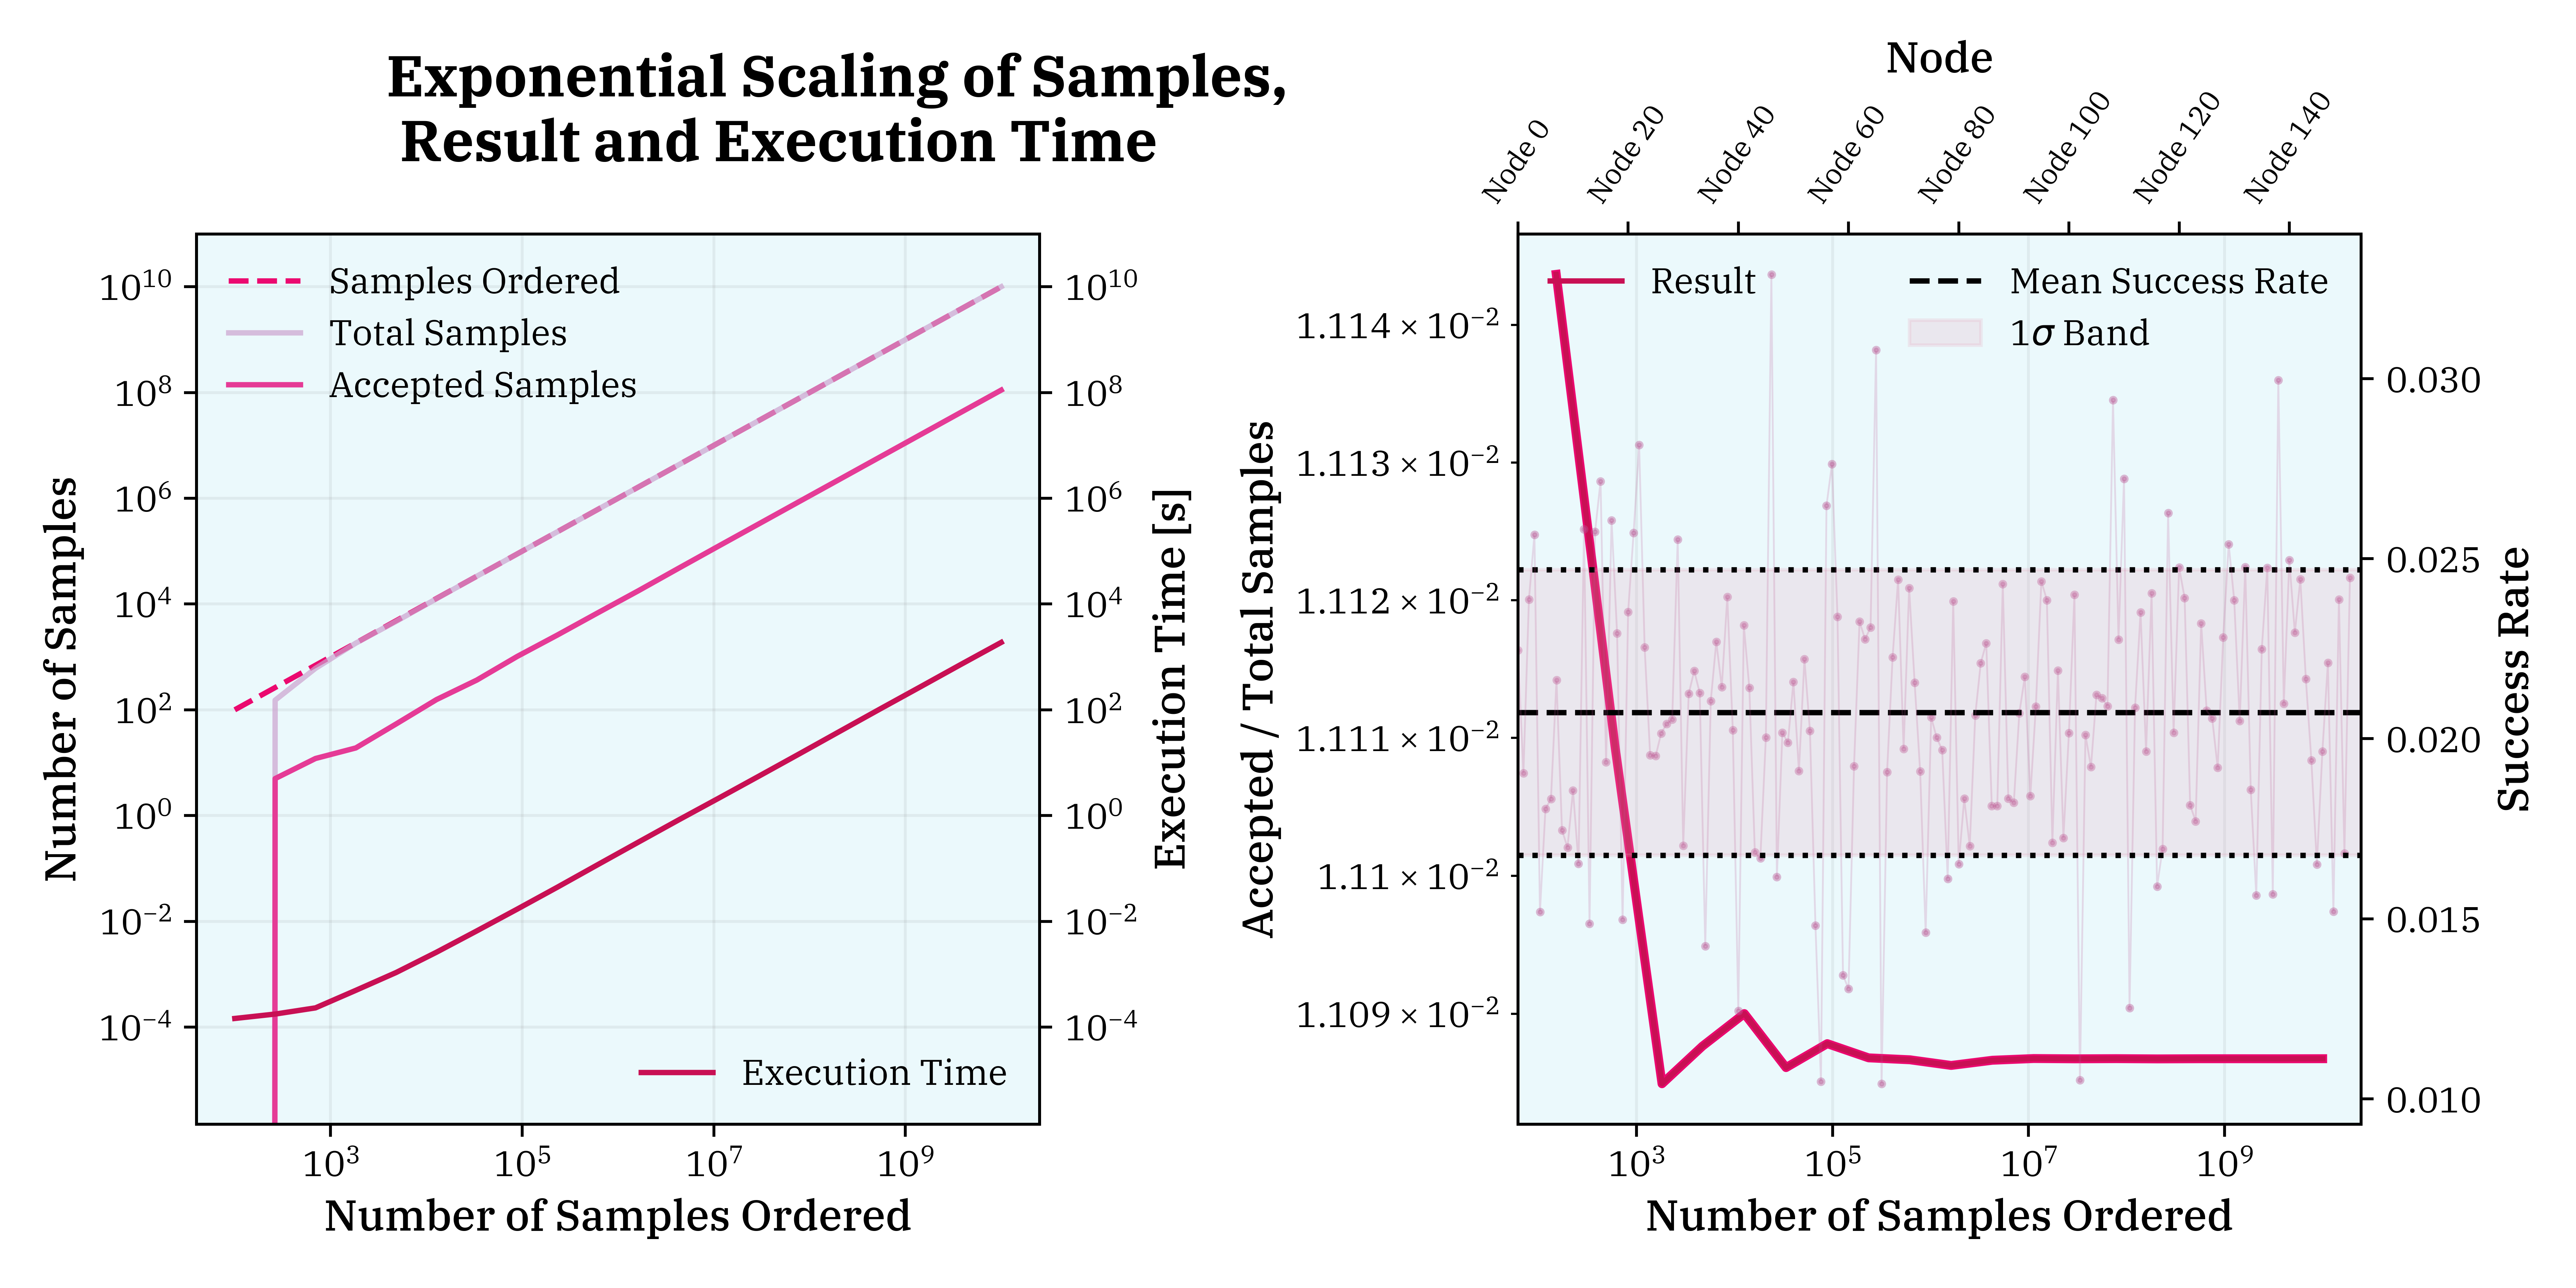
\includegraphics[width=\textwidth]{../StarShapes/Images/mass_const.png}
    \caption{Masa zvezdastega lika, ko je gostota konstantna.}
    \label{fig:mass_const}
\end{figure}

Na levi vidimo, kako se v log-log skali spreminja število vzorcev, kot se spreminja število vzorcev, ki jih 
sprejmemo. Pomembno je opaziti tudi naračanje časa izvajanja. Na desni vidimo, kako se vrednost mase spreminja,
dokler ne doseže konvergenco, za dovolj veliko število vzorcev. V ozadju pa je prikazana res CompSci metrika in 
sicer success rate, oz. kolikšen delež točk je bil znotraj območja, ki ga integriramo, v povprečju čez vse data 
point-e za različne zahtevane števila vzorcev. S tem lahko narišemo potem srednjo vrednost povprečne vrednosti mase
in njen ena-sigma interval. \\

Dodatno si lahko pogledamo še naključno naravo rezultatov, če si pogledamo raztros po posameznih procesorskih
jedrih. To je prikazano na sliki (\ref{fig:mass_const_heatmaps}). Na levi je prikazan rezultat, kjer je na $x$ 
osi $i$-to jedro, na $y$ osi pa je število zahtevanih vzorcev. Barva prikazuje maso, ki jo je vrnilo posamezno
jedro. Pričakovali oz. želeli bi, da so barve znotraj vrstice enake, kar pomeni, da je masa neodvisna od tega,
na katerem jedru se izvaja, ampak kot vidimo je nekaj naključnosti prisotne. Zanimivo mi je bilo potem še 
narisati čas izvajanja v istem formatu, kar je prikazano na desni. Barve se presenetljivo dobro ujemajo z manjšimi 
odstopanji. Lahko pa dobro oko opazi prvi namig sistemske napake, ki lahko kvari statistiko glede časa izvajanja 
na procesorsko jedro. Na levi strani desnega plota je viden malo temnejši pas, ki se pojavi na intervalu 
$i \in [8, 56]$. Ta efekt bo boljše viden na kasnejših slikah. Vmes pa lahko bralec ugiba, kaj bi lahko bil vzrok
za to. \\

\begin{figure}[H]
    \centering
    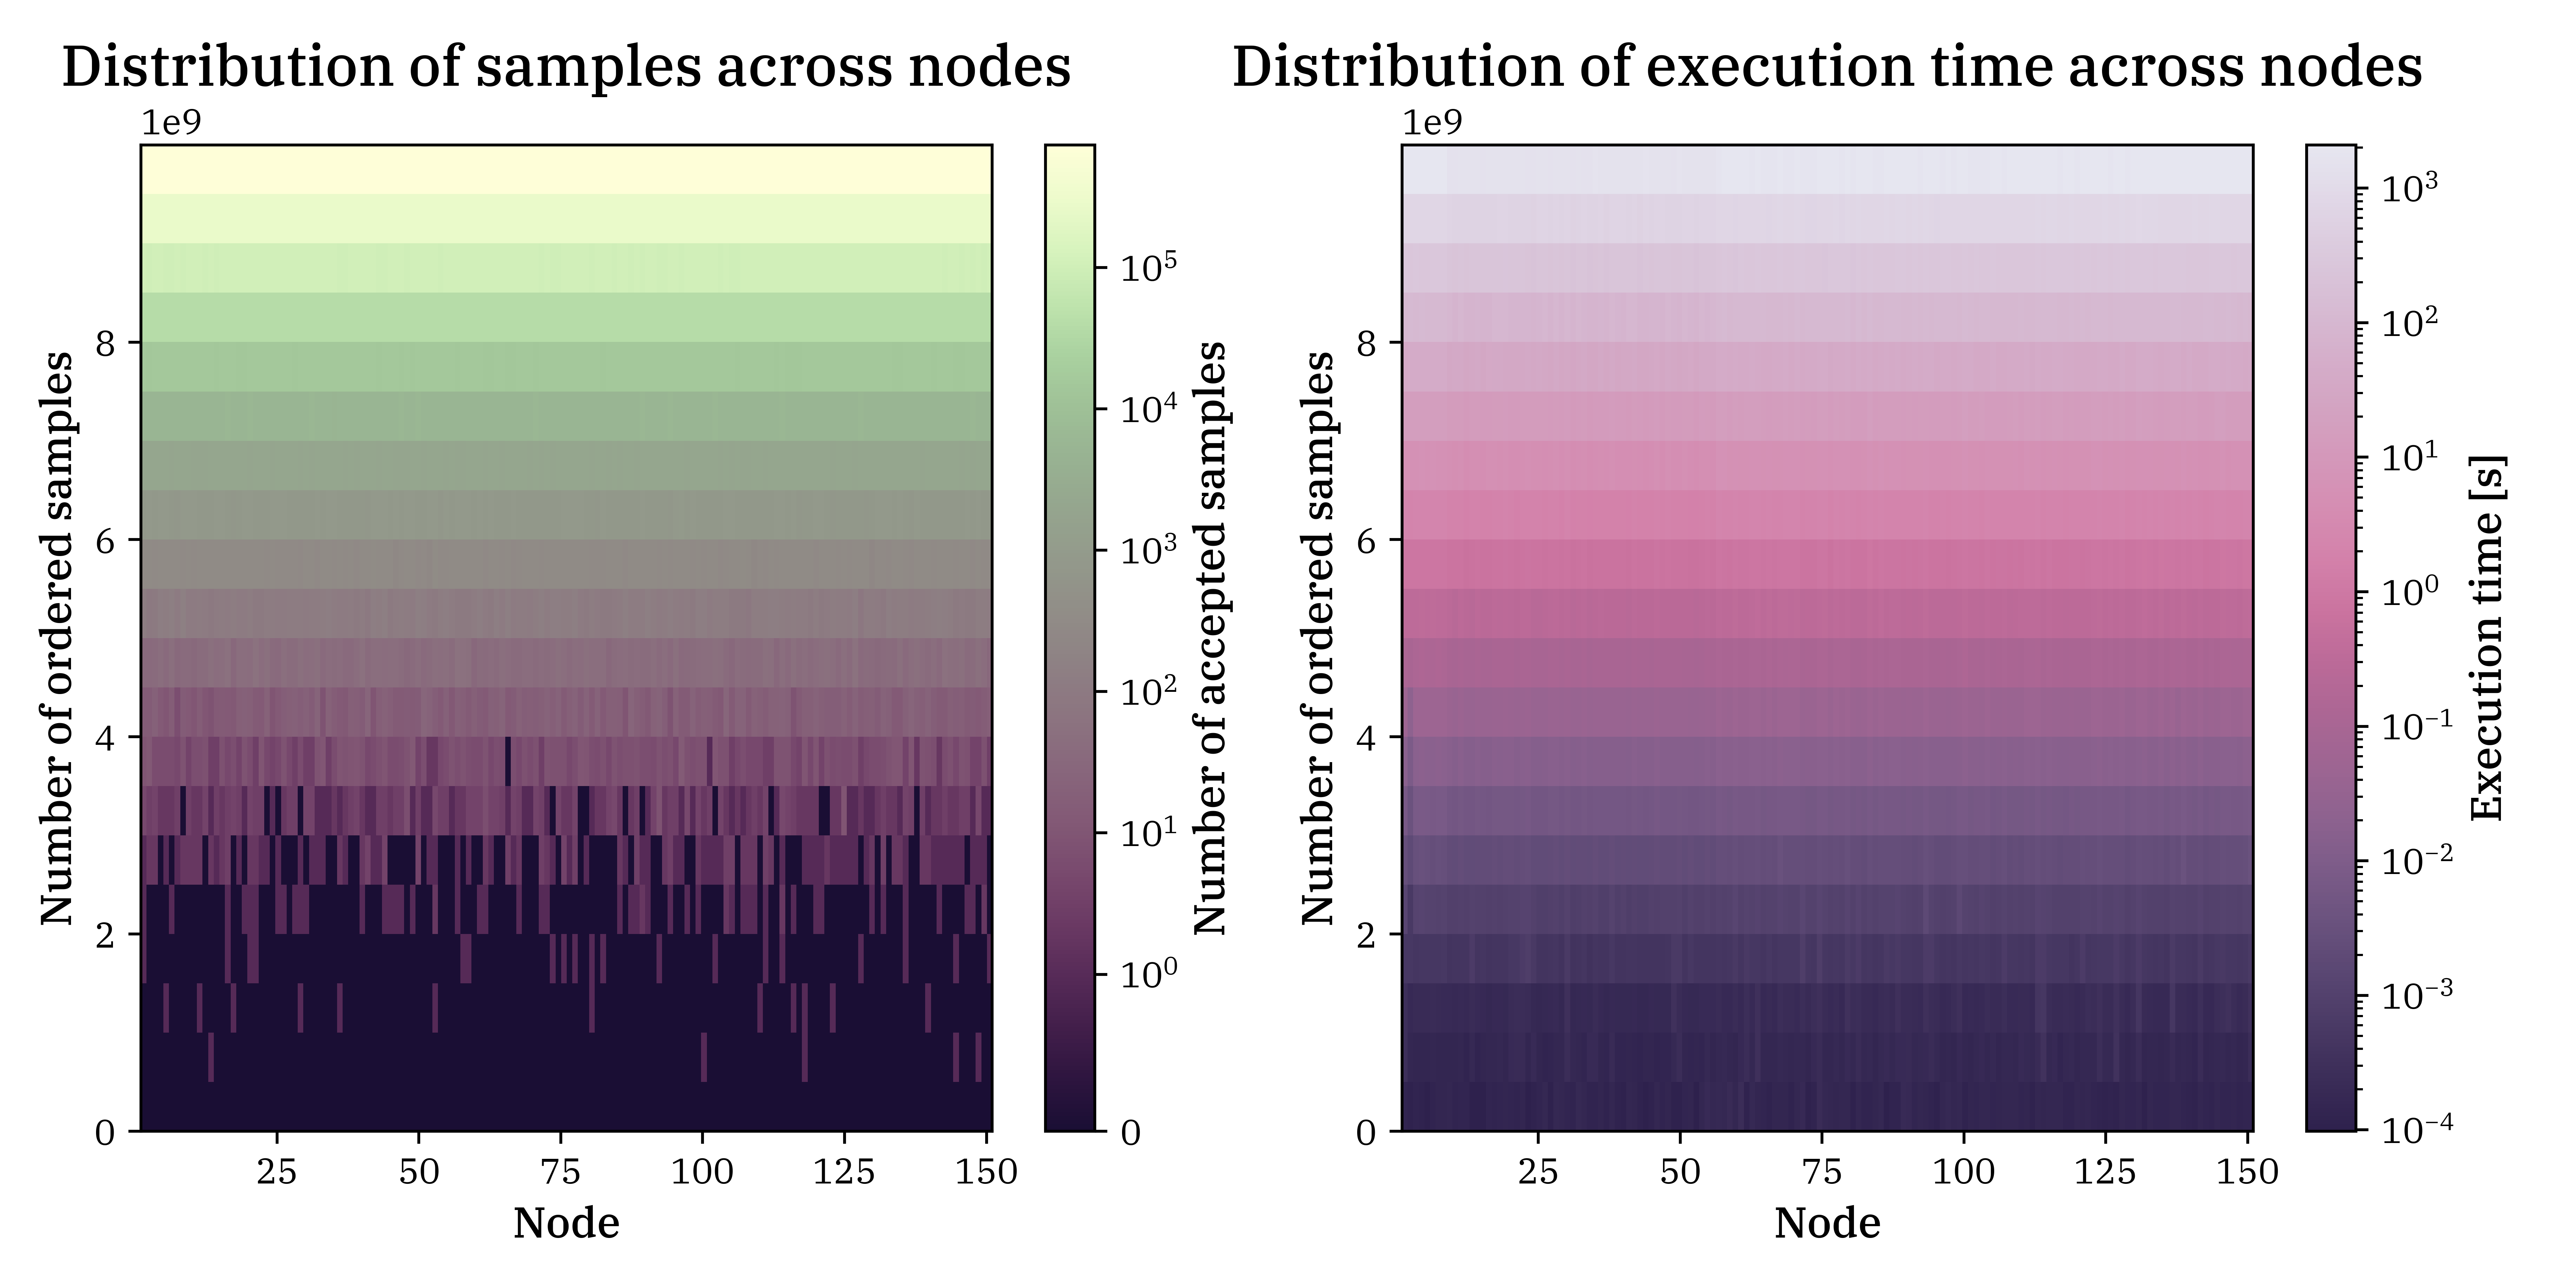
\includegraphics[width=\textwidth]{../StarShapes/Images/mass_const_heatmaps.png}
    \caption{Masa zvezdastega lika, ko je gostota konstantna.}
    \label{fig:mass_const_heatmaps}
\end{figure}

Sedaj pa si poglejmo še, kako se spreminja masa, ko je gostota odvisna od razdalje od izhodišča. Rezultati so
prikazani na sliki (\ref{fig:mass_radial}). Na levi je prikazana odvisnost mase od vrednosti $p$, ki je potenca
v radialnem profilu gostote. V ozadju je tokrat prikazan čas izvajanja v povprečju čez vsa jedra. Število vzorcev 
je bilo tu postavljeno na $10^7$. Na desni pa je prikazan success rate za različne vrednosti $p$ in njegov 
raztros po jedrih. Tukaj bi pričakovali, da dobimo popoln šum in res sure enough dobimo sliko, ki zgleda precej 
naključna. 

\begin{figure}[H]
    \centering
    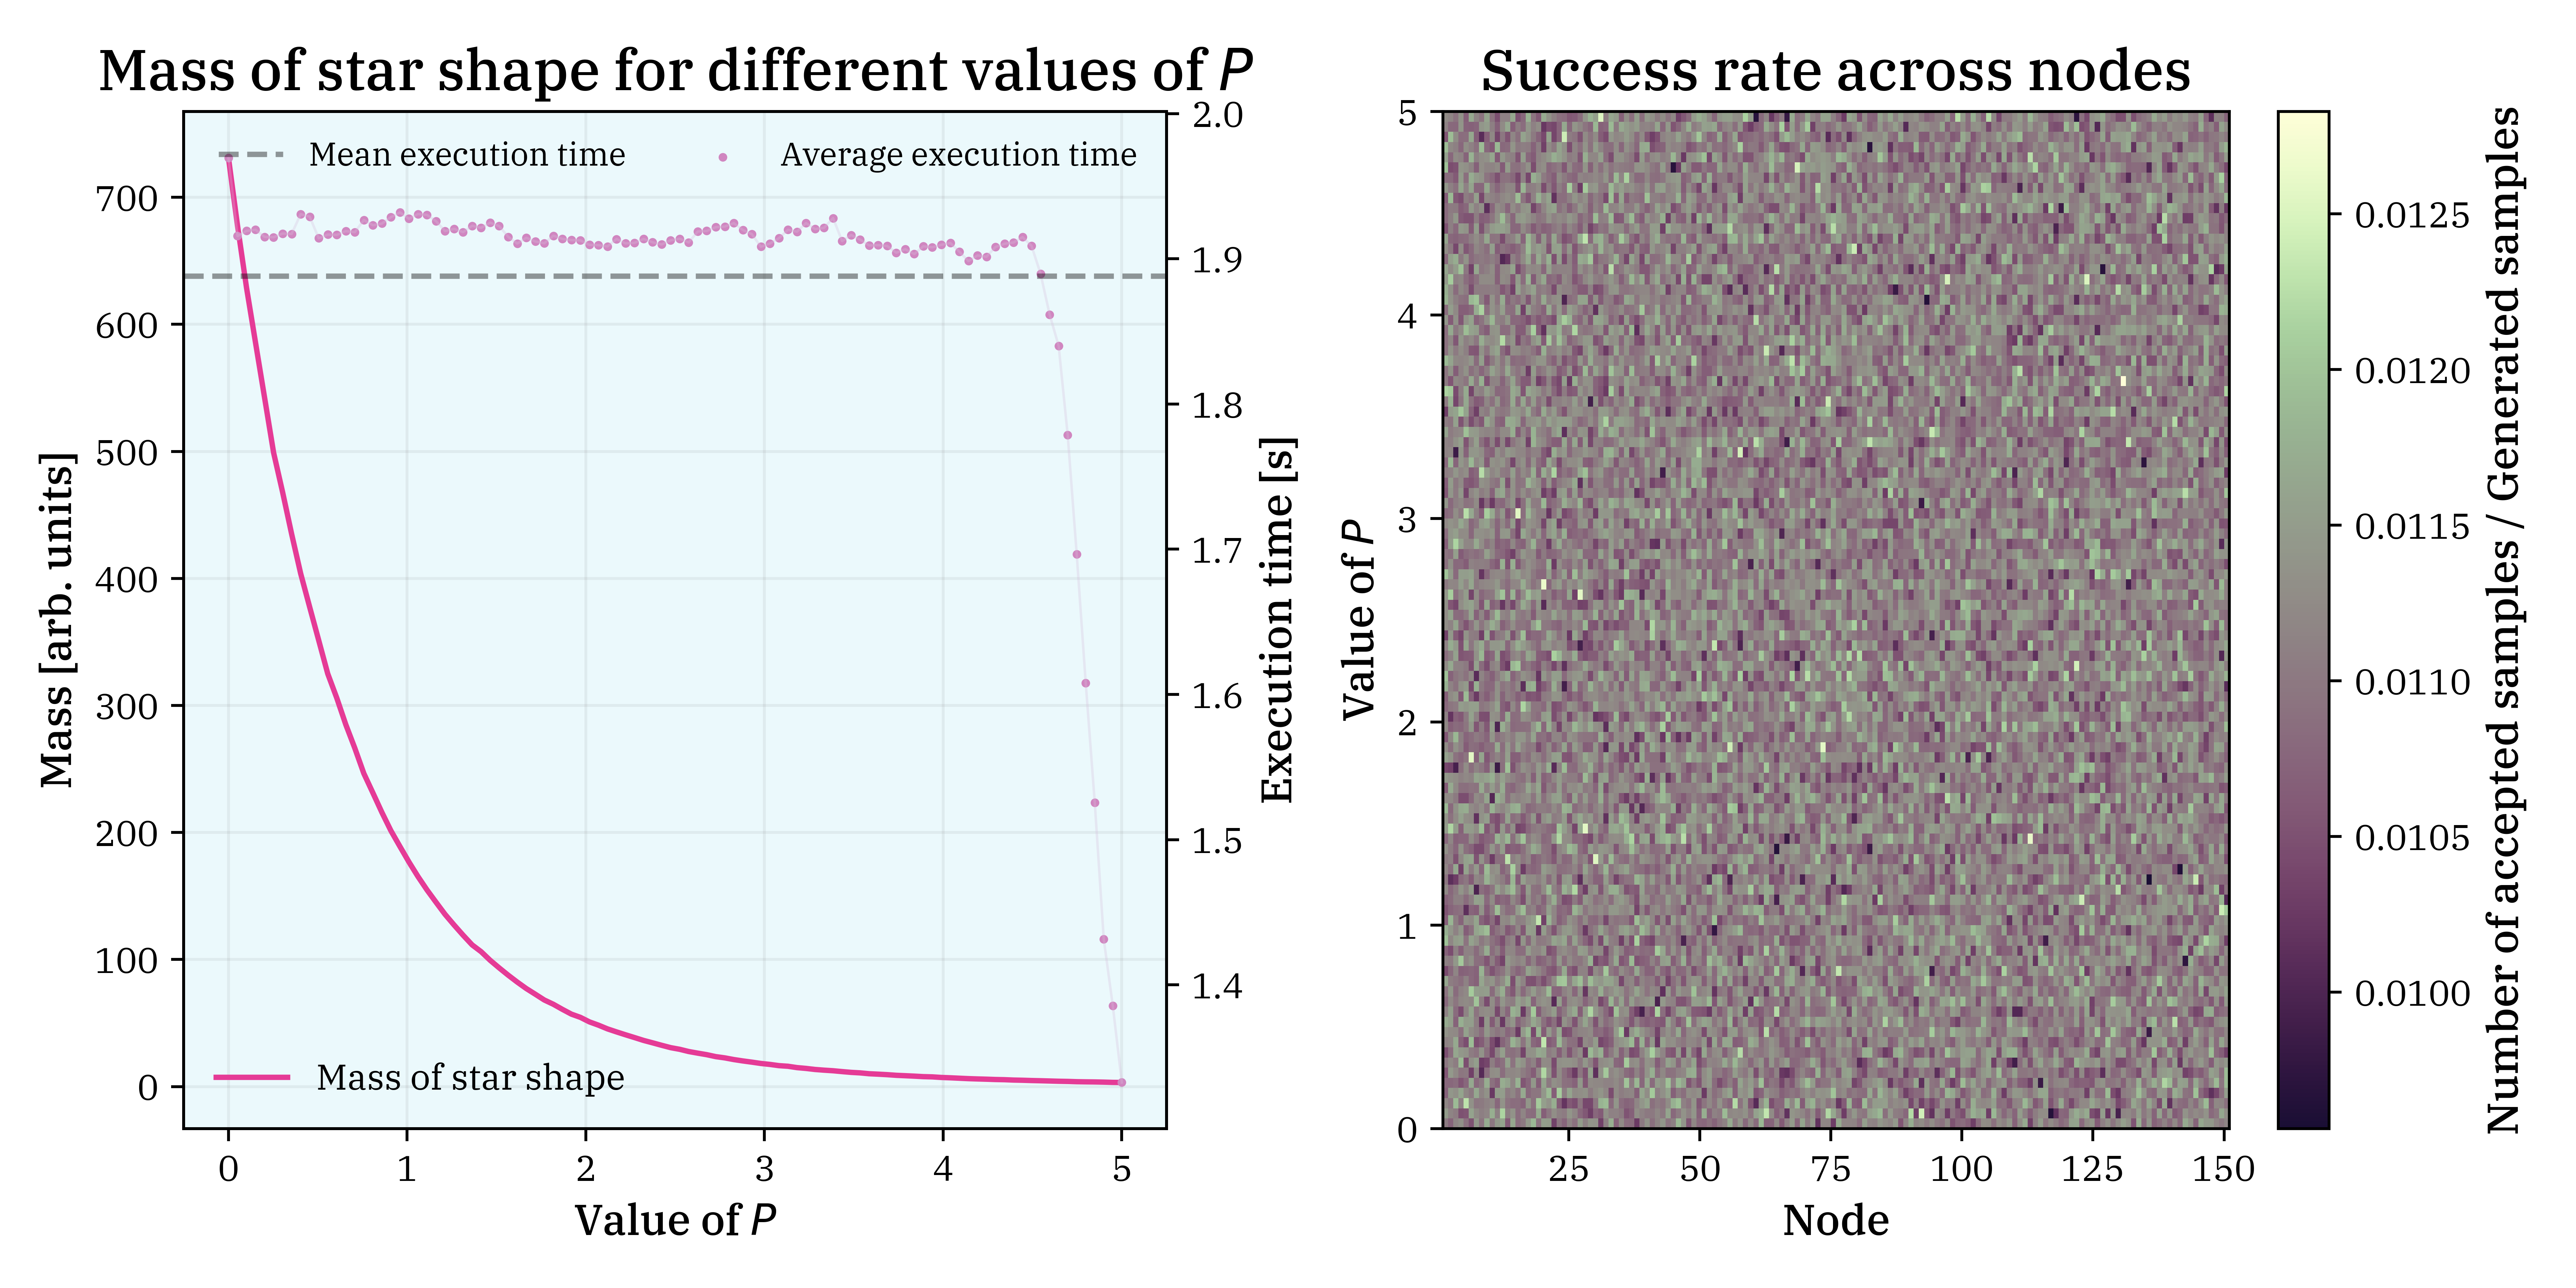
\includegraphics[width=\textwidth]{../StarShapes/Images/mass_radial.png}
    \caption{Masa zvezdastega lika, ko je gostota odvisna od razdalje od izhodišča.}
    \label{fig:mass_radial}
\end{figure}

Tako kot prej lahko pogledamo tudi tu raztros po jedrih, kar je prikazano na sliki (\ref{fig:mass_radial_heatmaps}).
Na levi je prikazan rezultat za maso, na desni pa za čas izvajanja. Na levi je zanimivo opaziti večje odstopanje
za večje vrednosti mase. To mi da misliti, da je mogoče relativna napaka pravzaprav konstantna in je tu napaka navidezno 
večja samo zaradi skale rezultata. Na desni strani pa človek prvo zagleda tisti efekt, ki sem ga omenil prej. Tu se izrazito
vidi pas, ki sem ga prej omenjal. To je posledica tega, da cluster ni idealiziran in sestavljen iz identičnih delov, ampak 
sta bili pri računanju uporabljeni dve mašini, ki imata boljše procesorje. Teh jeder je skupaj $48$. Čeprav sta na začetku clustra 
pride initial shift $8$ jeder od kontrolnega računalnika, ki je tu tudi računal. Pravzaprav, če bi pogledali side-by-side
Prvih $8$ jeder in potem preostanek od $56$ dalje, bi videli, da je prvih $8$ svetlejših, kar ge tu za tretjo vrsto 
procesorja, ki je najbolj.. recimo temu budget oriented. \\

\begin{figure}[H]
    \centering
    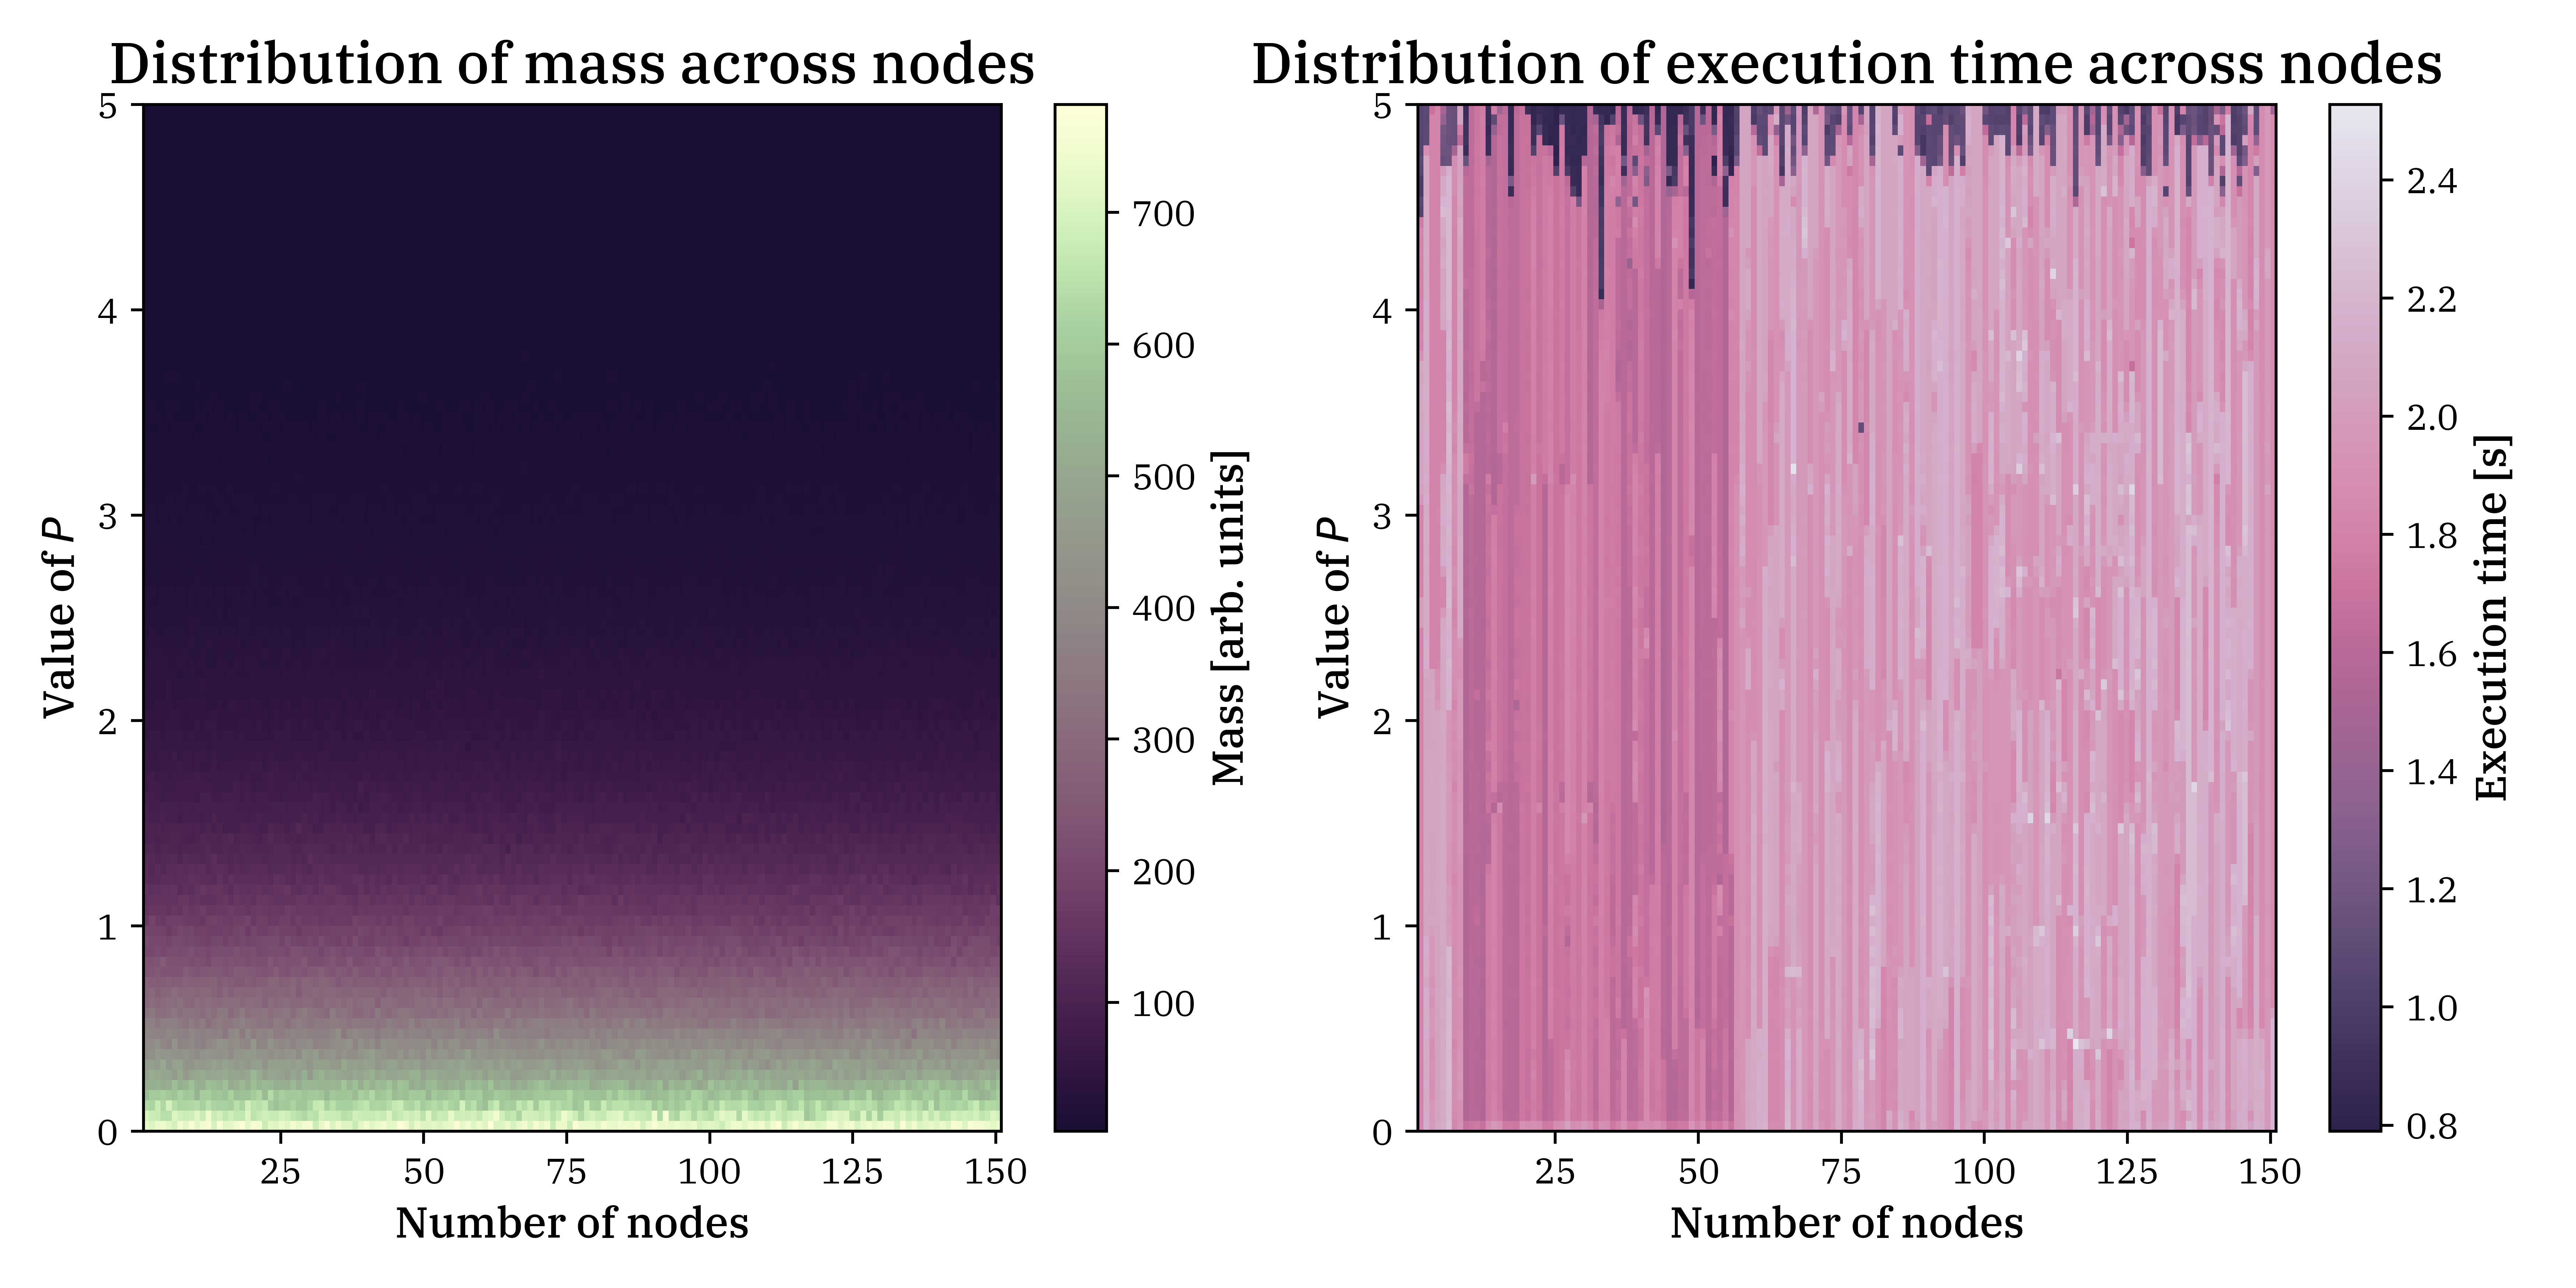
\includegraphics[width=\textwidth]{../StarShapes/Images/mass_radial_heatmaps.png}
    \caption{Masa zvezdastega lika, ko je gostota odvisna od razdalje od izhodišča.}
    \label{fig:mass_radial_heatmaps}
\end{figure}

Podobno se vsi ti efekti vidijo tudi pri izračunih za vztrajnostni moment. Ti so za konstantno vrednost gostote
prikazani na sliki (\ref{fig:angular_const}). Graf je zelo podoben tistemu za maso. Tudi vse količine na njemu so 
pravzaprav enake, z razliko tega, da je funkcija, ki jo integriramo drugačna.

\begin{figure}[H]
    \centering
    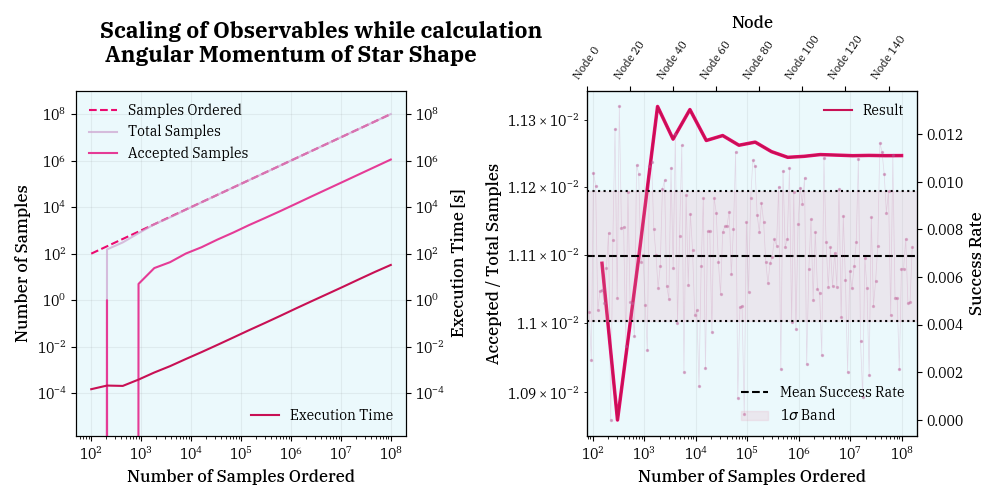
\includegraphics[width=\textwidth]{../StarShapes/Images/angular_const.png}
    \caption{Vztrajnostni moment zvezdastega lika, ko je gostota konstantna.}
    \label{fig:angular_const}
\end{figure}

Tudi tu sem iz radovednosti narisal še raztros po jedrih, kar je prikazano na sliki (\ref{fig:angular_const_heatmaps}).
Na levi je prikazan rezultat za vztrajnostni moment, na desni pa za čas izvajanja. Da se razlika med jedri boljše vidi, 
sem tu namesto vrtilne količine risal vrednost, ki je proporcionalna vrtilni količini; pravzaprav samo reskalacija, da 
so absolutne napake večje. Z risanjem relativne napake sem imel težave z postavitvijo normalizacije barve tako, da bi bile 
razlike lepo vidne po celem polju. Nekako na občutek pa se mi zdi, da je večja razlika v času izvajanja, kot pa v
pri masi, kljub temu, da ne bi smelo biti nobenega vpliva. Not sure. \\

\begin{figure}[H]
    \centering
    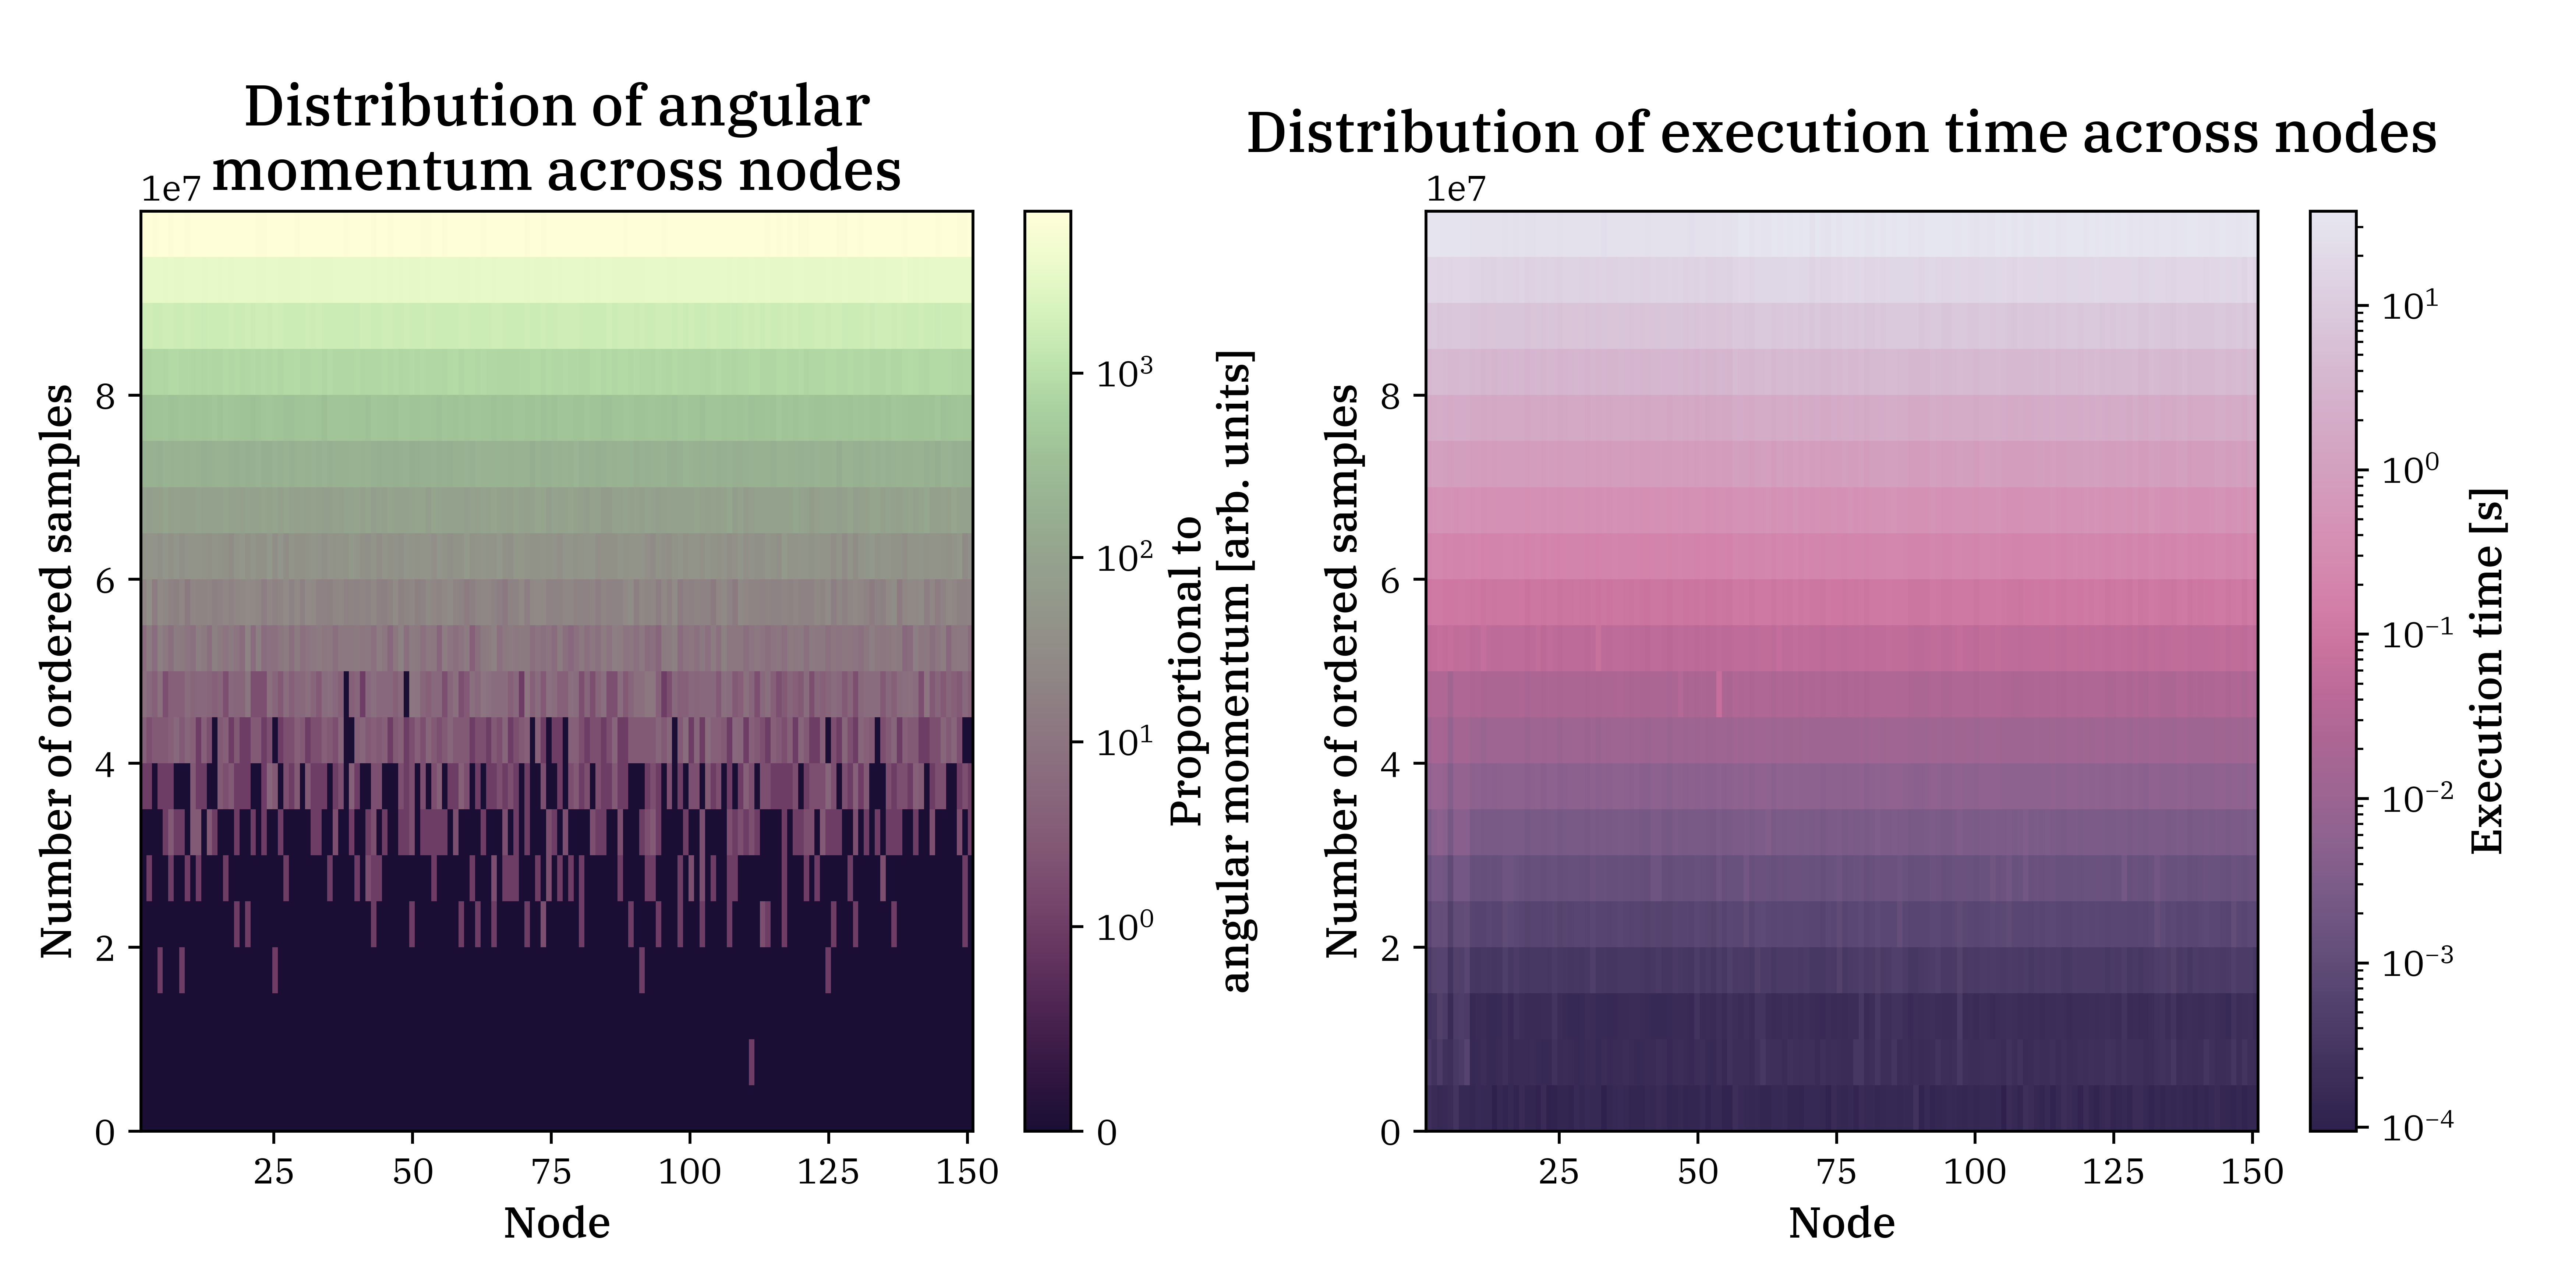
\includegraphics[width=\textwidth]{../StarShapes/Images/angular_const_heatmaps.png}
    \caption{Vztrajnostni moment zvezdastega lika, ko je gostota konstantna.}
    \label{fig:angular_const_heatmaps}
\end{figure}

Za primer, ko je gostota odvisna od razdalje od izhodišča, pa so rezultati prikazani na sliki (\ref{fig:angular_radial}).



\section{Komentarji in izboljšave}

\newpage
\bibliographystyle{unsrt}
\bibliography{sources}
\end{document}
